\documentclass[11pt]{article}

\usepackage[T1]{fontenc}
\usepackage{lmodern}
\usepackage[margin=1in]{geometry}
\usepackage{amsmath,amssymb,amsthm}
\usepackage{booktabs}
\usepackage{longtable}
\usepackage{microtype}
\usepackage[hidelinks]{hyperref}
\usepackage[round]{natbib}
\usepackage{xcolor}
\usepackage{multirow}
\usepackage{tikz}

\bibliographystyle{apalike}

\newcommand{\E}{\mathbb{E}}
\newcommand{\Prob}{\mathbb{P}}
\newcommand{\R}{\mathbb{R}}
\newcommand{\dw}{d_{W,K}}

\title{Wasserstein Causal Forests: Distribution-Valued Outcomes\\ under Covariate-Dependent Treatment Assignment}
\author{Hugo Gobato Souto\\ Dell Technologies\\ \texttt{hugo.souto@dell.com}}
\date{September 2026}

\begin{document}
\maketitle

\begin{abstract}
We propose Wasserstein Causal Forests (WCF) for observational studies in which each outcome is a probability distribution. WCF estimates the conditional law of potential quantile functions using particle boosting with shared treatment-arm partitions and monotone projection. An augmented inverse-propensity calibration step provides doubly robust scores for population and moderator-specific effects on distributional functionals. We introduce reference-distance effects that measure whether treatment moves the outcome distribution closer to a prespecified benchmark, and an optional two-part representation for a structural zero component. In simulations with covariate-dependent assignment and 1,000 training observations, reference-distance conditional-effect errors range from 0.030 to 0.046 for WCF, compared with 0.133 to 0.248 for Causal-DRF across three location and shape-effect regimes. Additional symmetric and nonlinear designs reveal variation in the ranking across estimands, with WCF at parity or better across the assignment mechanisms studied. A dedicated resolution study retained $K=25$ and $M=10$ after a pre-fixed stability rule failed; the larger $K=49$ grid improves full-range law error through extreme-tail coverage but ties on interior levels and costs more. The functional calibration is stable under a competent flexible (random-forest) propensity, while the default gradient-boosting factory is miscalibrated. The results support WCF as a conditional-law learner with functional calibration under observed confounding, while delimiting its performance under finite particle budgets and limited overlap.
\end{abstract}

\section{Introduction}\label{sec:intro}

Average treatment effects reduce an intervention to a difference in means, although many policy and scientific questions concern changes in dispersion, tail behavior, participation, or other features of an outcome law. Conditional distributional treatment effects formalize these questions by comparing potential-outcome distributions or functionals of those distributions. Recent work studies conditional distributional effects through kernel conditional mean embeddings and U-statistic regression \citep{CATEGeneralization}, counterfactual mean embeddings \citep{Counterfactualmeanembeddings}, robust regression of distributional effect pseudo-outcomes \citep{GRFDistributionalCausalEffects}, kernel treatment-effect tests \citep{martineztaboada2023efficient}, and distributional random forests \citep{DRF-paper,naf2026causaldrf}. These approaches establish a methodological basis for asking causal questions about outcomes whose distributional structure is scientifically relevant.

We study the related problem in which the observed outcome for each unit is itself a distribution-valued object, represented here by a quantile function on a common grid. The separation of outcomes, representations, and causal queries is also central to the TCDA framework \citep{souto_diamantis_tcda_2026}; here the representations are quantile coordinates and scalar distributional summaries. The Wasserstein geometry of quantile functions gives a natural metric for comparing such objects, while particle representations allow the conditional law of the quantile function to retain heterogeneity across units. The proposed Wasserstein Causal Forest combines this representation with a shared treatment-arm partition and a calibration step for scalar functionals of the law. The shared partition is intended for settings in which the treatment probability varies across covariates that also predict the potential-outcome law. The propensity score is the assignment probability $e(x)=\Pr(A=1\mid X=x)$ \citep{rosenbaum1983propensity}; covariate-dependent assignment becomes a source of confounding when those same covariates are prognostic and are not adequately adjusted for.

We study transformed average and conditional average treatment effects (TATE and TCATE), including two reference-distance estimands. Let $Q^a$ denote the potential-outcome quantile vector for a unit, let $q_\star$ be a prespecified reference quantile vector, and let $d_W$ denote the grid Wasserstein distance. The reference-adjusted marginal effect is
\[
\mathrm{TATE}_{\mathrm{ref}}
=\E\left[d_W(Q^1,q_\star)-d_W(Q^0,q_\star)\right],
\]
so a negative value indicates that treatment moves the unit-level outcome distribution closer to the reference on average. Its conditional analogue replaces the outer expectation by conditioning on $X=x$ or on a moderator stratum, giving a reference-adjusted TCATE. These contrasts express improvement or deterioration relative to a substantively chosen benchmark.

The contribution is threefold. First, WCF provides a concrete Wasserstein and quantile representation for conditional laws of distribution-valued outcomes. Second, it combines a common treatment-arm partition with a standard augmented inverse-propensity score for calibration of arbitrary reported functionals. The calibration is doubly robust in the usual nuisance-model sense for each functional when either the propensity nuisance or the corresponding conditional functional regression is consistently estimated \citep{bang2005doubly,chernozhukov2018double}. Third, the paper introduces the reference-adjusted TATE and TCATE contrasts and gives an optional two-part assembly for laws with an exact-zero component. The extension applies when some units have an entirely degenerate outcome distribution, as distinguished from individual zeros within a nondegenerate distribution.

We evaluate WCF in simulation studies designed to vary the treatment effect on location and distributional shape, the degree of overlap, the relationship between treatment assignment and prognostic covariates, and the presence of a point mass. The simulation programme now includes a resolution sensitivity study with common and interior 199-level targets and a family of assignment mechanisms separating linear, nonlinear, and prognosis-dependent assignment, with an alignment pair and a propensity-model check. The simulation design is stated directly in terms of the data-generating process. Income and wage distributions provide one interpretation of the quantile-valued outcome, but the same mathematical object can arise for regional expenditure distributions, health-care costs, benefit amounts, or any setting in which a unit is summarized by a distribution and an intervention acts on that distribution. For example, a regional income distribution may respond to a policy through changes in location, dispersion, or participation.

\section{The Wasserstein Causal Forest Model}\label{sec:model}

\subsection{Observed data, representation, and estimands}\label{sec:setup}

We observe independent units $O_i=(X_i,A_i,Q_i)$, where $X_i\in
\mathbb{R}^{d}$ is a vector of pre-treatment covariates, $A_i\in\{0,1\}$ is
the treatment indicator, and $Y_i$ is a probability distribution on $\mathbb{R}$ with finite second moment. We observe its quantile representation $Q_i=q_K(Y_i)$ on a
fixed grid $0<u_1<\cdots<u_K<1$. Writing $Q_Y$ for the quantile function of $Y$, the grid representation is
$q_K(Y)=(Q_Y(u_1),\ldots,Q_Y(u_K))\in\mathcal{Q}_K$, where
$\mathcal{Q}_K=\{q\in\mathbb{R}^K:q_1\leq\cdots\leq q_K\}$. Let
$w_k>0$ and $\sum_k w_k=1$. We use the weighted finite-grid geometry
\[
 d_{W,K}(q,q')=\left\{\sum_{k=1}^{K}w_k(q_k-q'_k)^2\right\}^{1/2}.
\]
This is a quadrature approximation to one-dimensional $W_2$
\citep{peyre2019optimaltransport}; all
estimands below refer to this finite-grid representation. It is also exactly the Wasserstein distance between the discrete distributions $\sum_k w_k\delta_{q_k}$ and $\sum_k w_k\delta_{q_k'}$. Sampling error in estimating each unit's quantile curve is outside the simulation design.

Write $Y^a$ for the potential outcome under treatment level $a$ and
$e(x)=\Pr(A=1\mid X=x)$ for the propensity score \citep{rosenbaum1983propensity}. The identification
conditions are consistency, conditional exchangeability
$Y^a\perp A\mid X$, and positivity $0<e(X)<1$ almost surely. Under these
conditions the arm-specific conditional law
\[
 P_a^K(x)=\operatorname{Law}\{q_K(Y^a)\mid X=x\}
 =\operatorname{Law}\{q_K(Y)\mid A=a,X=x\}
\]
is identified. The method estimates this law directly and subsequently
integrates measurable grid functionals against it.

For a measurable scalar functional $h:\mathcal{Q}_K\to\mathbb{R}$ satisfying $\mathbb{E}|h(q_K(Y^a))|<\infty$ for both arms, define
\[
 \mu_{a,h}(x)=\mathbb{E}\{h(q_K(Y^a))\mid X=x\},\qquad
 \theta_h=\mathbb{E}\{\mu_{1,h}(X)-\mu_{0,h}(X)\},
\]
and, for a pre-treatment moderator $V=g(X)$,
\[
 \tau_h(v)=\mathbb{E}\{\mu_{1,h}(X)-\mu_{0,h}(X)\mid V=v\}.
\]
We call $\theta_h$ the transformed average treatment effect (TATE) and
$\tau_h(v)$ the transformed conditional average treatment effect (TCATE).
For discrete moderators, only strata with positive population probability are considered.
The four functionals used in the experiments are
\begin{align*}
 h_{\mathrm{mean}}(q)&=\bar q=\sum_k w_kq_k,&
 h_{\mathrm{sd}}(q)&=\left\{\sum_k w_k(q_k-\bar q)^2\right\}^{1/2},\\
 h_{\mathrm{skew}}(q)&=\frac{\sum_k w_k(q_k-\bar q)^3}{h_{\mathrm{sd}}(q)^3},&
 h_{\mathrm{tail}}(q)&=\frac{\sum_{k>\lfloor K/2\rfloor}w_kq_k}{\sum_{k>\lfloor K/2\rfloor}w_k}.
\end{align*}
Skewness is assigned the value zero for a constant quantile vector; the upper-half functional includes the middle grid point when $K$ is odd.
Separately, the vector-valued identity
functional $h(q)=q$ gives the mean-quantile contrast
\[
 \tau_q(x)=\mathbb{E}\{q_K(Y^1)-q_K(Y^0)\mid X=x\},
\]
which is a vector-valued barycenter contrast and is distinct from nonlinear
outcome-level functionals of the barycenter.

The reference-distribution estimands use the scalar functional
\[
 h_{\mathrm{ref}}(q)=d_{W,K}(q,q_\star),
\]
where $q_\star$ is a fixed benchmark quantile vector. Thus
\[
 \theta_{\mathrm{ref}}=\mathbb{E}\{h_{\mathrm{ref}}(q_K(Y^1))
 -h_{\mathrm{ref}}(q_K(Y^0))\},\qquad
 \tau_{\mathrm{ref}}(v)=\mathbb{E}\{h_{\mathrm{ref}}(q_K(Y^1))
 -h_{\mathrm{ref}}(q_K(Y^0))\mid V=v\}.
\]
These are the reference-distance TATE and TCATE, respectively. A negative
value means that treatment moves the outcome law closer to the benchmark on
average within the relevant population. They are differences of expected
distances, not the distance between an expected quantile vector and the
benchmark.

Covariate-dependent treatment assignment can induce differences in the distribution of prognostic covariates between arms. Assignment may depend on the untreated mean, on covariates governing dispersion, or on other features of the potential-outcome laws. These are selection-on-observables mechanisms covered by conditional exchangeability. Dependence on unobserved potential-outcome information beyond $X$ requires additional identifying assumptions.

\subsection{Particle-law estimation}\label{sec:boosting}

For each arm, the fitted conditional law is an empirical particle law
\[
 \widehat P_{a,M}^K(x)=\frac{1}{M}\sum_{m=1}^{M}\delta_{p_{am}(x)},
 \qquad p_{am}(x)\in\mathcal{Q}_K.
\]
The particles are fitted by gradient boosting \citep{friedman2001greedy} on the collision-smoothed
energy score
\[
 S_\varepsilon(P,q)=\frac{1}{M}\sum_{m=1}^{M}d_{\varepsilon}(p_m,q)
 -\frac{1}{2M^2}\sum_{m,l=1}^{M}d_{\varepsilon}(p_m,p_l),
 \qquad
 d_{\varepsilon}(a,b)=\{d_{W,K}(a,b)^2+\varepsilon^2\}^{1/2}-\varepsilon.
\]
The unsmoothed energy score is strictly proper for probability laws on the weighted Euclidean space under a finite first-moment condition \citep{gneiting2007proper}. Finite particle count, smoothing, and the tree function class restrict the implemented optimization. The first term attracts the particle cloud to the observed quantile vector and
the second term preserves dispersion. At iteration $t$, only the observed arm contributes a gradient for unit $i$. The tree response for particle $m$ and coordinate $k$ is the preconditioned descent direction
\[
 G_{imk}=-\frac{M}{w_k}\frac{\partial S_\varepsilon(P,Q_i)}{\partial p_{mk}}
 \bigg|_{P=\widehat P_{A_i,M}^{K,(t)}(X_i)}.
\]
The shared tree maps $X_i$ to an arm-specific vector in $\mathbb{R}^{M K}$. For each arm, its update $g_a^{(t)}(x)$ produces
\[
 p_{am}^{(t+1)}(x)=\Pi_{\mathcal Q_K}^{w}\{p_{am}^{(t)}(x)+\eta_t g_{am}^{(t)}(x)\},
\]
where $\Pi_{\mathcal Q_K}^{w}$ is weighted isotonic projection, computed by the pool-adjacent-violators algorithm \citep{barlow1972isotonic}. A backtracking search halves $\eta_t$ until the observed-arm training score does not increase, up to numerical tolerance; fitting stops if no acceptable step is found. Prediction applies the fitted updates and projection in the same order.
The particle representation
estimates an arm-specific conditional law. It does not identify a coupling of
$Y^0$ and $Y^1$, and differences between matched particles from the two arms
are not individual treatment effects.

The final learner uses a shared covariate partition. Candidate splits are
scored with the pooled multi-output squared-error criterion and are retained
only when each child contains the required number of observations from each
arm. For the contrast-regularized update used in WCF, let $g_a$ be the
mean descent target in a leaf for arm $a$, let $n_a$ be its arm count, let
$\bar g=(n_0g_0+n_1g_1)/(n_0+n_1)$, and let $\delta=g_1-g_0$. With
$n_{\mathrm{eff}}=n_0n_1/(n_0+n_1)$ and
$c_\lambda=n_{\mathrm{eff}}/(n_{\mathrm{eff}}+\lambda)$, the leaf updates are
\[
 \widehat g_0=\bar g-\frac{n_1}{n_0+n_1}c_\lambda\delta,
 \qquad
 \widehat g_1=\bar g+\frac{n_0}{n_0+n_1}c_\lambda\delta.
\]
This shrinks the arm gap while preserving the count-weighted pooled gradient.
The strength $\lambda$ is selected from a fixed candidate set by held-out
energy risk computed only on each validation unit's observed arm. The method
initializes both arms with the same $M$ quantile vectors, selected at equally spaced ranks from the lexicographically ordered pooled training vectors. The common initialization starts the arm contrast at zero.

Figure~\ref{fig:pipeline} summarizes the two outputs of WCF.
\begin{figure}[t]
\centering
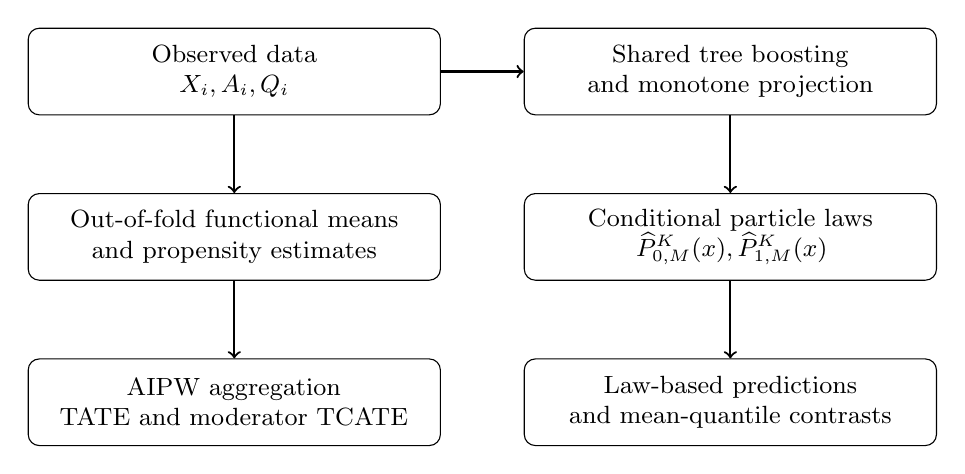
\begin{tikzpicture}[every node/.style={font=\small},box/.style={draw,rounded corners,align=center,text width=5cm,minimum height=1.1cm}]
\node[box] (data) at (0,0) {Observed data\\$X_i,A_i,Q_i$};
\node[box] (fit) at (6.3,0) {Shared tree boosting\\and monotone projection};
\node[box] (laws) at (6.3,-2.1) {Conditional particle laws\\$\widehat P_{0,M}^K(x),\widehat P_{1,M}^K(x)$};
\node[box] (nuisance) at (0,-2.1) {Out-of-fold functional means\\and propensity estimates};
\node[box] (effects) at (0,-4.2) {AIPW aggregation\\TATE and moderator TCATE};
\node[box] (lawoutputs) at (6.3,-4.2) {Law-based predictions\\and mean-quantile contrasts};
\draw[->,thick] (data) -- (fit);
\draw[->,thick] (data) -- (nuisance);
\draw[->,thick] (fit) -- (laws);
\draw[->,thick] (nuisance) -- (effects);
\draw[->,thick] (laws) -- (lawoutputs);
\end{tikzpicture}
\caption{WCF produces conditional laws and calibrated functional contrasts. The calibration uses out-of-fold particle fits and propensity estimates. It adjusts the functional contrasts without changing the final particle laws.}
\label{fig:pipeline}
\end{figure}


\subsection{Doubly robust calibration of scalar functionals}\label{sec:dr}

The particle law and the functional calibration layer target different
objects. For a declared functional $h$, let $\widehat m_{a,h}^{(-k)}(X_i)$
be the out-of-fold mean of $h$ over the fitted arm-$a$ particles, and let
$\widetilde e_i$ be a cross-fitted propensity estimate bounded away from zero and one. With $H_i=h(q_K(Y_i))$, define
\[
 \widehat\phi_i(h)=\widehat m_{1,h}^{(-k)}(X_i)
 -\widehat m_{0,h}^{(-k)}(X_i)
 +\frac{A_i}{\widetilde e_i}
   \{H_i-\widehat m_{1,h}^{(-k)}(X_i)\}
 -\frac{1-A_i}{1-\widetilde e_i}
   \{H_i-\widehat m_{0,h}^{(-k)}(X_i)\}.
\]
The marginal estimator is the sample mean of $\widehat\phi_i(h)$ and the
moderator-specific estimator is its sample mean within the observed bin
$V=v$. In the implementation, WCF applies this layer to the four grid
functionals and $h_{\mathrm{ref}}$. It replaces their reported contrast
columns, while the particle laws and all law-level scores remain those of the
particle booster.

The augmented score follows standard doubly robust estimation and cross-fitting \citep{bang2005doubly,chernozhukov2018double}. For fixed nuisance limits $m_a^\dagger(X)$ and $e^\dagger(X)$, let $\phi^\dagger(h)$ be the score with those limits substituted for the fitted nuisances. Writing $e^\dagger=e^\dagger(X)$ for brevity, its conditional bias is
\[
 \begin{aligned}
 &\mathbb{E}\{\phi^\dagger(h)\mid X\}-\{\mu_{1,h}(X)-\mu_{0,h}(X)\}\\
 &\qquad=(e^\dagger-e(X))\left[
 \frac{m_1^\dagger(X)-\mu_{1,h}(X)}{e^\dagger}
 +\frac{m_0^\dagger(X)-\mu_{0,h}(X)}{1-e^\dagger}
 \right].
 \end{aligned}
\]
Consequently, the score has the standard doubly robust property at the level
of the scalar functional: the bias vanishes when the propensity is correct or
when both arm-specific conditional means are correct, subject to positivity,
integrability, and the usual conditions controlling nuisance estimation and
cross-fitting. The robustness property applies to the calibrated averages; the conditional particle laws and pointwise mean-quantile contrasts remain outcome-model estimates. With fixed $M$, the functional means induced by a particle fit need not consistently approximate every chosen functional. The score identity therefore provides a robustness route, not a guarantee that the fixed-budget learner satisfies either nuisance-correctness condition.

The propensity nuisance may be estimated with any binary probability model whose predictions satisfy the required overlap and convergence conditions. Logistic regression is a working choice for the experiments. An empirical sensitivity check of the calibration under flexible propensity factories is reported in Section~\ref{sec:results-assignment}. Flexible classifiers can accommodate nonlinear assignment, with tuning confined to the appropriate training samples. Fixed propensity clipping can introduce bias when it excludes part of the true propensity range. Valid asymptotic inference additionally requires moment, nuisance-rate, and sample-splitting conditions; score unbiasedness alone is insufficient to establish efficiency.

\subsection{Optional two-part law for a degenerate component}\label{sec:zipt}

Some distribution-valued outcomes have a structural component in which the
entire unit-level outcome law is degenerate at a point. For example, a facility's expenditure distribution may be identically zero during an inactive period and nondegenerate during an active period. Participation and intensity are commonly separated in economic two-part models, including medical expenditure and count models \citep{duan1983medical,mullahy1986modified}. Here the mixture operates on distribution-valued observations: an atom at the all-zero quantile vector differs from a positive fraction of individuals with zero expenditure inside every unit's distribution. For such data, the optional two-part extension
estimates
\[
 \pi_a(x)=\Pr\{q_K(Y^a)\neq\mathbf{0}\mid X=x\}
\]
with an arm-specific binary classifier, fits the particle booster on the
nondegenerate rows, and assembles
\[
 \widehat P_a^{\mathrm{2p}}(x)=
 \{1-\widehat\pi_a(x)\}\delta_{\mathbf{0}}
 +\widehat\pi_a(x)\widehat P_{a,M}^{+,K}(x).
\]
The extension gives the degenerate component its own estimable probability
and lets every downstream law functional integrate over both parts. The plain
particle booster can place mass exactly at zero, but it has no
separate component-probability parameter and its particle masses are tied to
$1/M$; the two-part assembly makes that structural mass explicit. The extension can be enabled when the data contain this structural component. Its evaluation below concerns the assembled law and component probabilities; it does not assess an additional AIPW calibration of the mixture.
\section{Simulation studies}\label{sec:simulations}

The simulations examine conditional laws of quantile-valued outcomes under selection on observed covariates. We compare WCF with DRF and Causal-DRF in location and shape-effect designs, symmetric nonlinear designs, and a structural-zero mixture. Each replication uses the same training sample and independent test covariates across methods. The principal sample sizes are $n=500$ and $n=1000$, with ten replications per setting. Each test sample contains 1000 units. The moderator $V$ divides $X_1$ into four intervals with boundaries $-0.5$, $0$, and $0.5$.

\subsection{Location and shape-effect designs}\label{sec:income-design}

Covariates are independent $\mathrm{Unif}[-1,1]$ variables. For these designs $d=6$, and $A\mid X\sim\mathrm{Bernoulli}\{e(X)\}$. Potential quantile vectors follow
\begin{equation}\label{eq:dgp}
 Q_k^a=m_a(X)+\xi_a+\exp\{s_a(X)+\eta_a\}\psi\{z_k;\gamma_a(X)\},
 \qquad z_k=\Phi^{-1}\{(k-1/2)/K\},
\end{equation}
where
\[
 \psi(z;\gamma)=z+\gamma\left\{\frac{z^2-1}{2}+\frac{z^3-3z}{6}\right\}.
\]
Within each arm, $\xi_a\sim N(0,0.20^2)$ and $\eta_a\sim N(0,0.12^2)$ are independent of one another and of $X$. Assignment depends only on $X$. The function $\psi$ is increasing for $0\leq\gamma<1$, since its derivative is $1-\gamma+\gamma(z+1)^2/2$.

Define the baseline location, log-scale, and shape functions by
\begin{align*}
 b(x)&=0.55x_2+0.35x_3-0.45x_4+0.30x_5,\\
 s(x)&=0.16+0.08x_6-0.04x_2,\qquad
 g(x)=0.55+0.10x_4-0.08x_2,
\end{align*}
and let $C_{l,u}(t)=\min\{u,\max(l,t)\}$ and $\sigma(t)=(1+e^{-t})^{-1}$. The four designs are
\begin{align*}
\mathrm{IC0}:\quad &m_a=b,\quad s_a=s,\quad \gamma_a=C_{.05,.85}(g),\\
\mathrm{IC1}:\quad &m_a=b+a(0.20+0.15x_4),\quad s_a=s,\quad
 \gamma_a=C_{.05,.85}\{g-a(0.16+0.06x_4)\},\\
\mathrm{IC2}:\quad &m_a=b+a(0.10+0.05x_3),\quad s_a=s-0.12a,\quad
 \gamma_a=C_{.05,.85}(g-0.08a),\\
\mathrm{IC3}:\quad &(m_a,s_a,\gamma_a)\text{ as in IC1}.
\end{align*}
IC0 and IC1 use $e(x)=C_{.10,.90}\{\sigma(1.4x_4-1.1x_5+0.4x_6)\}$. IC2 uses $C_{.05,.95}\{\sigma(1.8x_4-0.9x_5)\}$, and IC3 uses $C_{.01,.99}[\sigma\{3.5(x_4-0.9x_5)\}]$. Thus IC0 has no treatment effect, IC1 changes location and shape, IC2 additionally changes scale, and IC3 reduces overlap while keeping IC1's outcome surfaces. The moderator $X_1$ does not enter the IC outcome or assignment surfaces, so the population TCATE is constant across its four bins in this family. The nonlinear designs below include effect modification by $X_1$. The reference vector is
\[
 q_{\star,k}=1.10+0.60\left[z_k+0.30\left\{\frac{z_k^2-1}{2}+\frac{z_k^3-3z_k}{6}\right\}\right].
\]
These equations describe a general location, scale, and shape construction. A regional income distribution is one possible interpretation, with treatment changing its location or dispersion and adoption depending on regional characteristics. The simulated curves are not constrained to be nonnegative, so this interpretation is illustrative rather than a calibrated model of income or expenditure.

\subsection{Symmetric and nonlinear designs}\label{sec:nonlinear-design}

The additional designs use $d=5$ independent uniform covariates and equation~\eqref{eq:dgp}, with reference $q_{\star,k}=z_k$. Define
\[
 f(x)=0.6\sin(\pi x_1)+0.4x_2x_3,\qquad
 e_m(x)=C_{.10,.90}[\sigma\{0.8(x_1+0.5x_2)\}].
\]
The conditional quantile contours are symmetric when $\gamma_a=0$, even though their locations and scales vary across units. D0 uses $m_a=f+0.8ax_1$, $s_a=0.20x_4+0.25ax_2$, $\gamma_a=0$, and zero latent shocks. D2 is a null-effect design with $m_a=f$, $s_a=0.20x_4$, $\gamma_a=0$, and independent normal shocks with standard deviations $(0.35,0.20)$.

D5 has equal mean quantile curves but different conditional laws. Its location is $m_a=f$ and $\gamma_a=0$. The control arm has $s_0=0.20x_4$ and shock standard deviations $(0.40,0.45)$; the treated arm has $s_1=0.20x_4+0.45^2/2$ and shock standard deviations $(0.15,0)$. The log-scale adjustment equates the expected scales. D6 uses $m_a=f+0.7ax_1$, $s_a=0.20x_4$, and $\gamma_a=0$, with $\eta_a\sim N(0,0.15^2)$ and
\[
 \xi_a\sim\tfrac12 N(-1.5,0.25^2)+\tfrac12 N(1.5,0.25^2).
\]
This creates a multimodal law of quantile curves while every realized curve retains a symmetric inner distribution. D7 changes shape: $m_a=f$, $s_a=0.20x_4$, $\gamma_a=0.20+0.10x_3+a(0.30+0.10x_1)$, and shock standard deviations $(0.35,0.20)$. These five designs use $e_m$.

D8 combines a smaller treatment effect with stronger confounding. It uses
\begin{align*}
 m_a(x)&=1.2\sin(\pi x_1)+0.9x_2x_3+a(0.12x_1+0.06),\\
 s_a(x)&=0.20x_4+0.05ax_2,\qquad \gamma_a(x)=0,\\
 e(x)&=C_{.05,.95}[\sigma\{2.5(x_1+0.7x_2-0.5x_3)\}],
\end{align*}
with shock standard deviations $(0.35,0.20)$. The nonlinear prognosis and covariate-dependent assignment in these designs allow the comparison to extend beyond the location and shape-effect family.

\subsection{Structural-zero designs}\label{sec:zi-design}

The four structural-zero designs use six independent uniform covariates. A unit's outcome vector is zero with probability $1-\pi_a(x)$ and otherwise follows equation~\eqref{eq:dgp} with
\begin{align*}
 m_a^+(x)&=4.80+0.35x_2-0.25x_4+a(\Delta+\beta x_2),\\
 s_a^+(x)&=0.10+0.06x_6-0.03x_2,\qquad
 \gamma_a^+(x)=C_{.05,.85}(0.50+0.06x_4-a\kappa).
\end{align*}
The normal shock standard deviations are $(0.15,0.10)$. The superscript $+$ denotes the nondegenerate branch; Gaussian shocks do not impose a strictly positive support. ZI0 and ZI1 use $(\Delta,\beta,\kappa)=(0,0,0)$, whereas ZI2 and ZI3 use $(0.28,0.08,0.10)$. ZI0 is a placebo and ZI2 changes only the nondegenerate component; both have $\pi_a(x)=C_{.05,.95}\{\sigma(1.2x_4-0.8x_2)\}$. ZI1 changes participation only, adding $a(0.90+0.20x_4)$ to this logistic index. These three designs use IC1's assignment mechanism. ZI3 changes both components and has
\[
 \pi_a(x)=C_{.01,.99}[\sigma\{3(x_4-0.9x_5)+a(0.90+0.60x_4)\}],
 \qquad e(x)=\pi_0(x).
\]
The reference vector is the same as in the IC family.

\subsection{Resolution sensitivity design}\label{sec:resolution-design}

The resolution study varies the budgets of the primary particle estimator while holding the data-generating process fixed at the four income regimes IC0 to IC3, at $n=1000$, and on seeds $0,\ldots,9$. Grid resolution is varied over $K\in\{5,25,49\}$ at $M=10$ and particle resolution over $M\in\{5,10,25\}$ at $K=25$. The one-factor slices are run first, each against the incumbent pair $(K,M)=(25,10)$. A full $3\times3$ factorial extension follows only if the one-factor slices show a material change, and it is allocated only to IC1 and IC3, the regime with a policy effect and the regime with the most difficult overlap. The forest comparators do not use $M$, so their resolution rows are repeated once per $K$ and are never duplicated across $M$.

The retention rule was fixed before the outcomes were inspected and is evaluated on the native-grid metrics of each cell. Write $R^{t}_{r}(K,M)$ for the between-seed mean WCF error on target $t\in\{\mathrm{ref},\mathrm{law}\}$ (reference-TCATE and conditional law) in regime $r$, and $\mathrm{SE}^{t}_{r}(K',M')$ for the between-seed standard error of the paired difference between $(K',M')$ and $(25,10)$. The incumbent pair $(25,10)$ is retained when every one-factor alternative $(K',M')\in\{(5,10),(49,10),(25,5),(25,25)\}$ satisfies
\begin{equation}\label{eq:sens-retention-rule}
\frac{\lvert R^{t}_{r}(K',M')-R^{t}_{r}(25,10)\rvert}{R^{t}_{r}(25,10)}\le 0.10,
\qquad t\in\{\mathrm{ref},\mathrm{law}\},\quad r\in\{\mathrm{IC1},\mathrm{IC3}\},
\end{equation}
and when no larger grid or particle count with $K'>25$ or $M'>25$ improves both targets by more than $2\,\mathrm{SE}^{t}_{r}(K',M')$ in both regimes. If the rule fails, the study reports the selected pair and the complete sensitivity table rather than silently changing the primary specification.

Because native-grid error targets change their estimand with $K$, the study also evaluates every fitted law on a common dense target. The common level set is
\begin{equation}\label{eq:sens-common-grid}
u_j=\frac{j-1/2}{199},\qquad j=1,\ldots,199,
\end{equation}
and particle coordinates and forest atoms are interpolated linearly in the quantile level, with constant continuation from the nearest endpoint outside the fitted grid, so no predicted value is extrapolated beyond the support of its own grid. The true data-generating curves and the regime reference vector are constructed directly on these levels from the regime specification, never interpolated from their coarse versions, and every method within a replication is evaluated against the same dense truth, test covariates, and evaluation bandwidth. A second interior level set $0.1+0.8u_j$ restricts the diagnostic to levels on which none of the proposed values $K\in\{5,25,49\}$ requires endpoint continuation, which separates tail coverage from the interior fit. Native-grid reference targets are regenerated on each cell's own $K$-grid; native, common, and interior targets are recorded under distinct identifiers and are never pooled.

The dense-grid calibrated functional effects use the interpolated particle clouds for the out-of-fold nuisance means and the interpolation of the observed coarse quantile curve for the observed functional values. This is a distinct information setting from a dense observed curve: the calibrated contrast targets the dense estimand while the observations remain coarse, so the augmentation identity is not exact at the dense level, and the interior reference targets inherit the same distinction. Native-grid calibrated effects are never relabelled as dense-grid effects.

The retained or selected pair is confirmed on fresh seeds $20,\ldots,39$ for $K\in\{25,49\}$ at $M=10$ over IC0 to IC3, with no reselection on those seeds. The confirmation is a stability check on twenty replications, not an equivalence test. Wall time and process peak memory are recorded for every cell. The study used seven concurrent single-thread workers, each pinned to one numerical thread, and the factorial extension was allocated only to IC1 and IC3.

\subsection{Assignment mechanisms and propensity models}\label{sec:assignment-design}

A second design family, labelled SYM, uses six independent $\mathrm{Unif}[-1,1]$ covariates and the generative form of equation~\eqref{eq:dgp}, but with a strictly symmetric inner law. Its outcome surfaces are
\begin{align*}
\mu(x)&=0.70\sin(\pi x_1)+0.35x_2x_3+0.20\cos(\pi x_4),\\
\tau(x)&=0.25+0.15\sin(\pi x_2),\\
s(x)&=0.12+0.08x_5^2-0.05x_3,
\end{align*}
with location $m_a(x)=\mu(x)+a\tau(x)$, log-scale $s_a(x)=s(x)$, shape coefficient $\gamma_a(x)=0$, no outer log-scale shock ($\eta_a\equiv 0$), and an outer location shock $\xi_a\sim N(0,0.25^2)$. Since $\psi(z;0)=z$, the arm law reduces to $q_k(Y^a)=\mu(X)+a\tau(X)+\xi_a+\exp\{s(X)\}z_k$, so the conditional quantile contour is pointwise symmetric in both arms: each coordinate $Q_k^a$ is symmetrically distributed about $\mu(X)+a\tau(X)+\exp\{s(X)\}z_k$, and $x_6$ enters no outcome surface.

Four assignment mechanisms share this outcome law. SYM-RANDOM uses the constant propensity $e(x)=0.5$. SYM-LIN uses the logistic link of a linear index, $e(x)=C_{.05,.95}\{\sigma(1.4x_1-1.1x_2+0.4x_3)\}$. SYM-NL uses a nonlinear propensity surface, $e(x)=C_{.05,.95}\{\sigma(1.6\sin(\pi x_1)+0.8x_2x_3-0.7x_4^2+0.35x_5)\}$. SYM-MU makes assignment a function of the baseline outcome location, $e(x)=C_{.05,.95}\{\sigma(1.2\mu(x)+0.5x_5)\}$. In all four cases the propensity is a function of pre-treatment covariates only, not of the potential outcomes; SYM-MU uses the baseline surface $\mu$ rather than the arm-specific law. Each mechanism has a null companion obtained by setting $\tau(x)=0$. The four mechanisms are fitted at $K=25$, $M=10$, ten seeds, and sample sizes $n\in\{500,1000\}$. The principal comparisons under SYM-LIN, SYM-NL, and SYM-MU are against the distributional forest comparators \citep{DRF-paper,naf2026causaldrf}, with SYM-RANDOM as a calibration control.

The alignment pair keeps the same outcome law and contrasts two nonlinear propensity indices with the same marginal law. SYM-ALIGN uses $e(x)=\sigma\{1.6\sin(\pi x_1)\}$ and SYM-IRREL uses $e(x)=\sigma\{1.6\sin(\pi x_6)\}$, where $x_6$ enters no outcome surface. Because the covariates are independent and identically distributed, the two propensity variables have the same marginal distribution by construction, so the pair isolates the relation between assignment and prognosis rather than the propensity spread. The alignment pair uses the same budgets and sample sizes as the four mechanisms, and null companions are included for both members.

Design checks on $200{,}000$ draws per regime confirm the intended overlap and balance before any estimator score is interpreted. Under SYM-NL the propensity ranges from $0.050$ to $0.932$ with treated fraction $0.4557$, and the largest standardized mean differences are $1.131$ for $\mu(X)$, $1.092$ for $\sin(\pi x_1)$, $0.819$ for $x_1$, and $0.212$ for $x_2x_3$. Under SYM-MU the propensity ranges from $0.131$ to $0.870$ with treated fraction $0.4992$, and the largest standardized mean differences are $0.615$ for $\mu(X)$, $0.574$ for $\sin(\pi x_1)$, $0.444$ for $x_1$, and $0.258$ for $x_5$. The nonlinear prognostic features carry the largest imbalances, which raw covariate means alone would not reveal. The generated inner laws pass the pointwise symmetry and monotonicity checks, with grid skewness at numerical precision (maximum absolute value $1.8\times10^{-15}$ across arms and regimes). The SYM-ALIGN and SYM-IRREL propensity marginals agree to a maximum absolute difference of $0.0018$.

The AIPW calibration layer accepts a binary-probability estimator factory that is fitted inside each training fold and returns probabilities on the same clipped scale. The default factory is the five-fold logistic regression with clipping to $[0.02,0.98]$ used in the primary fits. The propensity sensitivity adds a random-forest factory (200 trees, minimum leaf size 5, single-threaded), a gradient-boosting factory at the library defaults, and an oracle diagnostic that substitutes the true propensity; the oracle is a diagnostic benchmark and is explicitly not a feasible competitor. All sensitivity fits use three outcome folds and contrast candidates $\{0,50,500\}$, holding the outcome learner, $K$, $M$, seeds, and test designs fixed. The random-forest and gradient-boosting factories use no held-out tuning beyond their fixed settings, so their contrasts measure the propensity model family rather than a tuned alternative, and the comparison under nonlinear assignment is a misspecification stress test that does not by itself establish the doubly robust property.


\subsection{Comparators and implementation}\label{sec:implementation}

DRF estimates the conditional outcome distribution with separate forests for the two arms \citep{DRF-paper}. Causal-DRF uses a shared treatment-aware splitting criterion designed for the conditional kernel treatment effect \citep{naf2026causaldrf}. Both return arm-specific weights on observed training quantile vectors. The comparisons use the authors' implementations, with 2500 trees per arm for DRF and 2500 trees for Causal-DRF, organized in groups of 50 trees. WCF is the particle estimator with functional calibration described in Section~\ref{sec:model}. The structural-zero comparison uses its optional two-part law estimator.

All reported models use the uniform midpoint grid with $K=25$, and WCF uses $M=10$ particles. The boosting budget is 100 iterations, initial step size $0.12$, maximum tree depth 4, minimum total leaf size 10, minimum arm leaf size 5, and smoothing constant $\varepsilon=10^{-3}$. The backtracking search permits twelve halvings and accepts score changes within $10^{-12}$ numerical tolerance. Contrast shrinkage is selected from $\{0,50,500\}$ by observed-arm validation risk, with ties favoring larger penalties. The IC fits use three-fold outcome fitting and selection; the nonlinear and two-part fits use two folds. Propensity estimation uses five-fold logistic regression, with probabilities clipped to $[0.02,0.98]$. This interval excludes part of IC3's true propensity range, so the fitted propensity is not exactly specified in that design even if its untruncated logistic index were known. The mixture probability is fitted with separate logistic classifiers using an $\ell_2$ penalty with inverse strength $C=1$; these classifiers are fitted on the full training arm. Quantile vectors with maximum absolute coordinate at most $10^{-12}$ are classified as degenerate.

The selected outcome penalty is reused for the out-of-fold calibration fits; its selection is not nested within each calibration training fold. Consequently, the out-of-fold predictions exclude each observation from tree fitting but not from penalty selection. The simulations evaluate point-estimation accuracy and do not invoke asymptotic confidence-interval guarantees for this tuning arrangement. The fixed $K$ and $M$ are computational choices; a dedicated sensitivity study retains $K=25$ and $M=10$. The sensitivity study uses three outcome folds and contrast candidates $\{0,50,500\}$ for every design and is reported in Sections~\ref{sec:resolution-design} and~\ref{sec:assignment-design}.

\subsection{Evaluation}\label{sec:metrics}

We evaluate the mean-quantile contrast $\tau_q(x)$ by the root mean squared error over all test units and all $K$ coordinates. For each scalar functional, TCATE error is the RMSE over the four moderator bins, using the bin average of the true conditional contrast on the test covariates. TATE error is the absolute error in the marginal contrast averaged over those test covariates. For WCF, the recorded marginal predictions average the training-bin AIPW estimates using the test sample's bin frequencies. They therefore evaluate a test-standardized bin estimator, rather than the direct training-sample AIPW mean. Training and test covariates are sampled from the same population. The reference-distance TATE and TCATE use $h_{\mathrm{ref}}$ with the same aggregation rules.

For concise comparisons, functional TATE and TCATE errors are averaged over the four functionals within each replication. Since these functionals have different units, these averages are descriptive summaries whose values depend on the stated outcome scale. Appendix~\ref{app:functional-results} reports each functional separately. Each table gives the mean replication error and its between-replication standard error, after averaging arm-specific or functional-specific entries within the replication. Thus the marginal-effect columns report mean absolute error, not root mean squared error over replications.

Conditional-law error is squared maximum mean discrepancy \citep{gretton2012kernel}, computed with a Gaussian kernel on $(\sqrt{w_k}q_k)_k$. The bandwidth is chosen by a median-distance rule on the quadrature truth nodes, identically across methods within each arm and replication. This bandwidth is used for evaluation only. Law scores average the first 200 test units in each arm and then average the two arms. Oracle expectations use a product Gauss--Hermite rule with twelve nodes per nondegenerate normal shock, separately weighted across mixture components. Accordingly, the law discrepancy is evaluated against the quadrature approximation to the true law.

In the structural-zero designs, mass error is the RMSE between the true zero-component probability and the predicted mass on vectors with maximum absolute coordinate at most $0.05$. The mass-contrast metric is the RMSE of the corresponding treatment contrast over moderator bins. The explicit atom in the two-part model contributes its estimated mixture weight to this probability. All error criteria are oriented so that smaller values indicate greater accuracy.

\section{Results}\label{sec:results}

\subsection{Location and shape-effect designs}

Tables~\ref{tab:revision-income-500} and~\ref{tab:revision-income-1000} report both sample sizes. WCF has the smallest mean error in every displayed column. At $n=1000$, its reference-distance TCATE error is $0.0300$ in IC1, $0.0330$ in IC2, and $0.0463$ in IC3, compared with $0.1333$, $0.1567$, and $0.2476$ for Causal-DRF. Its conditional-law errors also remain lower in these three designs. The IC0 placebo yields smaller false effects for WCF on the mean-quantile, functional, and reference-distance contrasts. The per-functional results in Appendix~\ref{app:functional-results} qualify the aggregate ranking: for example, the forests estimate the grid-standard-deviation effects more accurately in several IC settings. These comparisons establish performance differences under the stated assignment and outcome mechanisms; they do not isolate a single architectural cause of the differences.

\begin{table}[t]
\centering
\scriptsize
\setlength{\tabcolsep}{3pt}
\caption{Location and shape-effect designs at $n=500$. Entries are mean(SE) over ten replications. MeanQ is quantile-vector RMSE; Law is squared MMD. TATE columns give mean absolute error and TCATE columns give mean bin RMSE. Functional errors are averaged within each replication.}
\label{tab:revision-income-500}
\begin{tabular}{llrrrrrr}
\toprule
DGP & Method & MeanQ & Law & TATE & TCATE & Ref. TATE & Ref. TCATE \\
\midrule
IC0 & WCF & 0.0503(0.0149) & 0.0205(0.0006) & 0.0143(0.0024) & 0.0384(0.0029) & 0.0245(0.0042) & 0.0496(0.0043) \\
IC0 & Causal-DRF & 0.2323(0.0117) & 0.0651(0.0018) & 0.1371(0.0065) & 0.1374(0.0064) & 0.1869(0.0109) & 0.1870(0.0108) \\
IC0 & DRF & 0.2339(0.0102) & 0.0905(0.0021) & 0.1356(0.0058) & 0.1356(0.0058) & 0.1857(0.0100) & 0.1858(0.0100) \\
IC1 & WCF & 0.1427(0.0116) & 0.0236(0.0010) & 0.0175(0.0022) & 0.0444(0.0025) & 0.0294(0.0059) & 0.0522(0.0051) \\
IC1 & Causal-DRF & 0.2109(0.0114) & 0.0627(0.0023) & 0.1157(0.0061) & 0.1162(0.0061) & 0.1563(0.0102) & 0.1566(0.0101) \\
IC1 & DRF & 0.2194(0.0101) & 0.0821(0.0022) & 0.1188(0.0056) & 0.1189(0.0056) & 0.1611(0.0098) & 0.1612(0.0097) \\
IC2 & WCF & 0.0987(0.0173) & 0.0220(0.0011) & 0.0115(0.0022) & 0.0360(0.0034) & 0.0185(0.0027) & 0.0387(0.0049) \\
IC2 & Causal-DRF & 0.2328(0.0115) & 0.0685(0.0016) & 0.1420(0.0061) & 0.1423(0.0061) & 0.1860(0.0107) & 0.1862(0.0106) \\
IC2 & DRF & 0.2495(0.0127) & 0.0978(0.0023) & 0.1520(0.0067) & 0.1520(0.0067) & 0.2016(0.0121) & 0.2016(0.0121) \\
IC3 & WCF & 0.1415(0.0078) & 0.0251(0.0010) & 0.0290(0.0046) & 0.0550(0.0033) & 0.0285(0.0064) & 0.0668(0.0066) \\
IC3 & Causal-DRF & 0.3444(0.0113) & 0.0773(0.0019) & 0.1950(0.0063) & 0.1954(0.0063) & 0.2662(0.0110) & 0.2666(0.0109) \\
IC3 & DRF & 0.3688(0.0107) & 0.0958(0.0029) & 0.2082(0.0057) & 0.2083(0.0057) & 0.2834(0.0101) & 0.2836(0.0101) \\
\bottomrule
\end{tabular}
\end{table}

\begin{table}[t]
\centering
\scriptsize
\setlength{\tabcolsep}{3pt}
\caption{Location and shape-effect designs at $n=1000$. Entries are mean(SE) over ten replications, using the same metrics as Table~\ref{tab:revision-income-500}.}
\label{tab:revision-income-1000}
\begin{tabular}{llrrrrrr}
\toprule
DGP & Method & MeanQ & Law & TATE & TCATE & Ref. TATE & Ref. TCATE \\
\midrule
IC0 & WCF & 0.0356(0.0054) & 0.0153(0.0005) & 0.0100(0.0012) & 0.0240(0.0025) & 0.0142(0.0025) & 0.0298(0.0028) \\
IC0 & Causal-DRF & 0.1947(0.0081) & 0.0467(0.0010) & 0.1134(0.0048) & 0.1138(0.0047) & 0.1570(0.0081) & 0.1572(0.0080) \\
IC0 & DRF & 0.1963(0.0063) & 0.0641(0.0013) & 0.1104(0.0038) & 0.1105(0.0038) & 0.1543(0.0065) & 0.1544(0.0065) \\
IC1 & WCF & 0.0904(0.0061) & 0.0174(0.0006) & 0.0128(0.0015) & 0.0271(0.0020) & 0.0143(0.0028) & 0.0300(0.0032) \\
IC1 & Causal-DRF & 0.1760(0.0090) & 0.0455(0.0009) & 0.0962(0.0051) & 0.0966(0.0051) & 0.1329(0.0080) & 0.1333(0.0080) \\
IC1 & DRF & 0.1876(0.0058) & 0.0591(0.0012) & 0.1012(0.0032) & 0.1013(0.0032) & 0.1394(0.0056) & 0.1395(0.0056) \\
IC2 & WCF & 0.0700(0.0034) & 0.0167(0.0006) & 0.0099(0.0016) & 0.0255(0.0016) & 0.0143(0.0033) & 0.0330(0.0035) \\
IC2 & Causal-DRF & 0.1975(0.0072) & 0.0488(0.0010) & 0.1176(0.0039) & 0.1179(0.0039) & 0.1565(0.0069) & 0.1567(0.0069) \\
IC2 & DRF & 0.2298(0.0063) & 0.0724(0.0016) & 0.1357(0.0034) & 0.1358(0.0034) & 0.1795(0.0050) & 0.1796(0.0050) \\
IC3 & WCF & 0.1103(0.0043) & 0.0180(0.0006) & 0.0188(0.0027) & 0.0412(0.0030) & 0.0161(0.0042) & 0.0463(0.0064) \\
IC3 & Causal-DRF & 0.3177(0.0076) & 0.0605(0.0013) & 0.1784(0.0043) & 0.1786(0.0042) & 0.2474(0.0067) & 0.2476(0.0067) \\
IC3 & DRF & 0.3481(0.0055) & 0.0773(0.0014) & 0.1972(0.0033) & 0.1973(0.0033) & 0.2701(0.0051) & 0.2702(0.0051) \\
\bottomrule
\end{tabular}
\end{table}


\subsection{Symmetric and nonlinear designs}

Table~\ref{tab:revision-abstract} shows a more varied ranking. WCF has the smallest mean conditional-law error in D0, D2, D5, D7, and D8. In contrast, both forest baselines have smaller reference-distance TCATE error in D2, D5, D6, D7, and D8. Thus improved law approximation under the kernel metric does not ensure improved estimation of every scalar functional. D5 illustrates the distinction: the two potential outcomes have identical mean quantile curves but different conditional laws, so the causal questions depend on the functional chosen.

The multimodal D6 design is particularly challenging for WCF. Its law error is $0.0178$, compared with $0.0064$ for Causal-DRF and $0.0059$ for DRF. Its reference-distance TCATE error is also larger. This result limits claims of general superiority under covariate-dependent assignment and motivates further investigation of the particle representation in multimodal settings.

\begin{table}[t]
\centering
\scriptsize
\setlength{\tabcolsep}{3pt}
\caption{Symmetric and nonlinear designs at $n=1000$. Entries are mean(SE) over ten replications, using the same metrics as Table~\ref{tab:revision-income-500}.}
\label{tab:revision-abstract}
\begin{tabular}{llrrrrrr}
\toprule
DGP & Method & MeanQ & Law & TATE & TCATE & Ref. TATE & Ref. TCATE \\
\midrule
D0 & WCF & 0.0868(0.0021) & 0.0234(0.0015) & 0.0041(0.0005) & 0.0101(0.0005) & 0.0038(0.0006) & 0.0097(0.0008) \\
D0 & Causal-DRF & 0.1391(0.0012) & 0.1033(0.0036) & 0.0230(0.0017) & 0.0512(0.0013) & 0.0087(0.0012) & 0.0886(0.0023) \\
D0 & DRF & 0.1672(0.0022) & 0.1191(0.0041) & 0.0131(0.0010) & 0.0415(0.0012) & 0.0048(0.0016) & 0.0799(0.0023) \\
D2 & WCF & 0.0410(0.0057) & 0.0098(0.0003) & 0.0137(0.0022) & 0.0300(0.0024) & 0.0115(0.0037) & 0.0399(0.0032) \\
D2 & Causal-DRF & 0.0818(0.0052) & 0.0154(0.0003) & 0.0292(0.0043) & 0.0340(0.0039) & 0.0151(0.0053) & 0.0227(0.0048) \\
D2 & DRF & 0.0627(0.0028) & 0.0138(0.0003) & 0.0130(0.0024) & 0.0230(0.0025) & 0.0140(0.0053) & 0.0224(0.0052) \\
D5 & WCF & 0.0946(0.0153) & 0.0220(0.0008) & 0.0146(0.0039) & 0.0332(0.0024) & 0.0202(0.0040) & 0.0418(0.0055) \\
D5 & Causal-DRF & 0.0765(0.0032) & 0.0374(0.0008) & 0.0187(0.0038) & 0.0302(0.0027) & 0.0144(0.0034) & 0.0239(0.0025) \\
D5 & DRF & 0.0917(0.0036) & 0.0431(0.0011) & 0.0132(0.0029) & 0.0295(0.0030) & 0.0151(0.0037) & 0.0235(0.0028) \\
D6 & WCF & 0.2189(0.0178) & 0.0178(0.0008) & 0.0506(0.0127) & 0.0970(0.0147) & 0.0191(0.0063) & 0.0862(0.0094) \\
D6 & Causal-DRF & 0.2310(0.0132) & 0.0064(0.0004) & 0.0504(0.0090) & 0.0845(0.0084) & 0.0261(0.0075) & 0.0585(0.0091) \\
D6 & DRF & 0.1986(0.0099) & 0.0059(0.0003) & 0.0461(0.0077) & 0.0852(0.0052) & 0.0220(0.0060) & 0.0501(0.0068) \\
D7 & WCF & 0.0553(0.0030) & 0.0094(0.0003) & 0.0162(0.0021) & 0.0368(0.0024) & 0.0156(0.0045) & 0.0386(0.0034) \\
D7 & Causal-DRF & 0.0721(0.0034) & 0.0129(0.0003) & 0.0208(0.0039) & 0.0360(0.0032) & 0.0128(0.0042) & 0.0235(0.0033) \\
D7 & DRF & 0.0662(0.0031) & 0.0142(0.0003) & 0.0156(0.0027) & 0.0353(0.0027) & 0.0135(0.0043) & 0.0238(0.0037) \\
D8 & WCF & 0.0635(0.0020) & 0.0127(0.0003) & 0.0234(0.0044) & 0.0672(0.0070) & 0.0377(0.0098) & 0.0793(0.0117) \\
D8 & Causal-DRF & 0.2100(0.0082) & 0.0417(0.0007) & 0.0706(0.0072) & 0.0889(0.0047) & 0.0325(0.0088) & 0.0584(0.0077) \\
D8 & DRF & 0.1623(0.0056) & 0.0416(0.0008) & 0.0257(0.0033) & 0.0509(0.0039) & 0.0446(0.0113) & 0.0724(0.0081) \\
\bottomrule
\end{tabular}
\end{table}


\subsection{Structural-zero outcomes}

Table~\ref{tab:revision-zi} compares the two-part WCF law estimator with the two forest baselines. The two-part estimator has the smallest mean mass-placement and law errors across the four designs. In ZI3, its mass error is $0.0598$, compared with $0.1731$ for Causal-DRF and $0.3475$ for DRF; its law error is $0.0176$, compared with $0.0768$ and $0.2472$. Its mass-contrast errors are also lower in the reported comparison. These results concern estimation of the structural mixture and its participation contrast. The two-part fits do not include the functional AIPW calibration, and no double-robustness claim is attached to these mass or law scores.

\begin{table}[t]
\centering
\scriptsize
\setlength{\tabcolsep}{3pt}
\caption{Structural-zero outcomes at $n=1000$. Entries are mean(SE) over ten replications. Zero mass and mass contrast are RMSEs; Law is squared MMD. Two-part WCF estimates the mixture without AIPW functional calibration.}
\label{tab:revision-zi}
\begin{tabular}{llrrr}
\toprule
DGP & Method & Zero mass & Mass contrast & Law \\
\midrule
ZI0 & Two-part WCF & 0.0537(0.0032) & 0.0427(0.0092) & 0.0133(0.0007) \\
ZI0 & Causal-DRF & 0.0945(0.0026) & 0.0595(0.0054) & 0.0247(0.0013) \\
ZI0 & DRF & 0.1058(0.0029) & 0.0561(0.0079) & 0.0296(0.0013) \\
ZI1 & Two-part WCF & 0.0526(0.0033) & 0.0365(0.0055) & 0.0154(0.0011) \\
ZI1 & Causal-DRF & 0.0901(0.0029) & 0.0426(0.0087) & 0.0249(0.0012) \\
ZI1 & DRF & 0.1022(0.0037) & 0.0479(0.0080) & 0.0291(0.0016) \\
ZI2 & Two-part WCF & 0.0537(0.0032) & 0.0427(0.0092) & 0.0136(0.0007) \\
ZI2 & Causal-DRF & 0.0946(0.0026) & 0.0597(0.0051) & 0.0258(0.0014) \\
ZI2 & DRF & 0.1060(0.0030) & 0.0564(0.0080) & 0.0304(0.0013) \\
ZI3 & Two-part WCF & 0.0598(0.0032) & 0.0445(0.0074) & 0.0176(0.0010) \\
ZI3 & Causal-DRF & 0.1731(0.0039) & 0.2051(0.0082) & 0.0768(0.0028) \\
ZI3 & DRF & 0.3475(0.0079) & 0.3823(0.0130) & 0.2472(0.0099) \\
\bottomrule
\end{tabular}
\end{table}


\subsection{Resolution sensitivity}\label{sec:results-resolution}

The resolution study varies the grid size $K\in\{5,25,49\}$ at $M=10$ and the particle budget $M\in\{5,10,25\}$ at $K=25$ around the primary pair $(25,10)$ at $n=1000$, following the resolution design of Section~\ref{sec:resolution-design}. The pre-fixed retention rule of equation~\eqref{eq:sens-retention-rule} failed for the incumbent pair. On seeds $0,\ldots,9$, the native reference-TCATE error in IC1 is $15.5$ percent smaller at $K=5$ and $14.1$ percent smaller at $K=49$ than at $K=25$, while $K=5$ is $19.1$ percent larger on native law error, and no larger pair improves both targets by more than two between-seed standard errors in both IC1 and IC3. Table~\ref{tab:sensitivity-km} reports the one-factor slices, and the rule returned no automatic selection, so the study reports the complete sensitivity table rather than changing the primary specification silently.

\begin{table}[t]
\centering
\scriptsize
\setlength{\tabcolsep}{3pt}
\caption{Sensitivity of WCF to the quantile grid size $K$ and the particle budget $M$ at $n=1000$ for designs IC0 to IC3. Panel A varies $K$ at $M=10$; Panel B varies $M$ at $K=25$. Entries are mean(SE) over ten replications. The native reference TCATE is evaluated on each cell's own $K$-grid, while the common and interior columns are evaluated on fixed 199-level targets. The primary setting $(K,M)=(25,10)$ appears in both panels.}
\label{tab:sensitivity-km}
\begin{tabular}{llrrrrr}
\toprule
\multicolumn{7}{l}{\textit{Panel A: $K$ sensitivity at $M=10$}} \\
DGP & $K$ & Ref. TCATE native & Law common & Ref. TCATE common & Law interior & Ref. TCATE interior \\
\midrule
IC0 & 5 & 0.0318(0.0027) & 0.2751(0.0030) & 0.0321(0.0030) & 0.0256(0.0007) & 0.0321(0.0031) \\
IC0 & 25 & 0.0286(0.0026) & 0.0669(0.0009) & 0.0286(0.0026) & 0.0178(0.0006) & 0.0292(0.0034) \\
IC0 & 49 & 0.0297(0.0034) & 0.0358(0.0006) & 0.0298(0.0034) & 0.0172(0.0007) & 0.0316(0.0037) \\
IC1 & 5 & 0.0261(0.0026) & 0.2474(0.0028) & 0.0249(0.0027) & 0.0280(0.0008) & 0.0248(0.0029) \\
IC1 & 25 & 0.0309(0.0026) & 0.0605(0.0009) & 0.0290(0.0028) & 0.0195(0.0007) & 0.0317(0.0030) \\
IC1 & 49 & 0.0265(0.0024) & 0.0342(0.0007) & 0.0242(0.0024) & 0.0196(0.0007) & 0.0270(0.0031) \\
IC2 & 5 & 0.0302(0.0036) & 0.2434(0.0029) & 0.0519(0.0051) & 0.0265(0.0006) & 0.0313(0.0036) \\
IC2 & 25 & 0.0310(0.0035) & 0.0605(0.0010) & 0.0342(0.0042) & 0.0198(0.0008) & 0.0315(0.0034) \\
IC2 & 49 & 0.0333(0.0033) & 0.0340(0.0006) & 0.0330(0.0037) & 0.0191(0.0005) & 0.0335(0.0035) \\
IC3 & 5 & 0.0531(0.0059) & 0.2454(0.0027) & 0.0542(0.0058) & 0.0297(0.0011) & 0.0582(0.0058) \\
IC3 & 25 & 0.0474(0.0061) & 0.0621(0.0010) & 0.0505(0.0066) & 0.0228(0.0010) & 0.0506(0.0067) \\
IC3 & 49 & 0.0512(0.0055) & 0.0361(0.0008) & 0.0534(0.0055) & 0.0231(0.0010) & 0.0526(0.0058) \\
\midrule
\multicolumn{7}{l}{\textit{Panel B: $M$ sensitivity at $K=25$}} \\
DGP & $M$ & Ref. TCATE native & Law common & Ref. TCATE common & Law interior & Ref. TCATE interior \\
\midrule
IC0 & 5 & 0.0298(0.0028) & 0.0674(0.0010) & 0.0298(0.0028) & 0.0173(0.0006) & 0.0297(0.0037) \\
IC0 & 10 & 0.0286(0.0026) & 0.0669(0.0009) & 0.0286(0.0026) & 0.0178(0.0006) & 0.0292(0.0034) \\
IC0 & 25 & 0.0280(0.0026) & 0.0661(0.0009) & 0.0282(0.0026) & 0.0174(0.0006) & 0.0295(0.0033) \\
IC1 & 5 & 0.0300(0.0032) & 0.0613(0.0009) & 0.0280(0.0032) & 0.0202(0.0007) & 0.0320(0.0035) \\
IC1 & 10 & 0.0309(0.0026) & 0.0605(0.0009) & 0.0290(0.0028) & 0.0195(0.0007) & 0.0317(0.0030) \\
IC1 & 25 & 0.0281(0.0031) & 0.0602(0.0009) & 0.0259(0.0033) & 0.0197(0.0006) & 0.0289(0.0036) \\
IC2 & 5 & 0.0330(0.0035) & 0.0607(0.0010) & 0.0344(0.0036) & 0.0192(0.0007) & 0.0330(0.0035) \\
IC2 & 10 & 0.0310(0.0035) & 0.0605(0.0010) & 0.0342(0.0042) & 0.0198(0.0008) & 0.0315(0.0034) \\
IC2 & 25 & 0.0339(0.0038) & 0.0608(0.0013) & 0.0345(0.0041) & 0.0198(0.0010) & 0.0331(0.0040) \\
IC3 & 5 & 0.0463(0.0064) & 0.0614(0.0008) & 0.0493(0.0066) & 0.0226(0.0009) & 0.0498(0.0062) \\
IC3 & 10 & 0.0474(0.0061) & 0.0621(0.0010) & 0.0505(0.0066) & 0.0228(0.0010) & 0.0506(0.0067) \\
IC3 & 25 & 0.0487(0.0066) & 0.0618(0.0012) & 0.0526(0.0062) & 0.0233(0.0011) & 0.0534(0.0061) \\
\bottomrule
\end{tabular}
\end{table}


Because native-grid targets change with $K$, the resolution evidence is read together with targets evaluated on the fixed common 199-level and interior level sets of Section~\ref{sec:resolution-design}. The $K=49$ full-range law error reduction of roughly $42$ to $46$ percent is a tail-coverage effect: a $K=25$ fit is continued as a constant outside its fitted support, whereas a $K=49$ fit reaches further into the extreme quantile levels. On the interior levels $0.1$ to $0.9$ the two grids are statistically indistinguishable, with all paired $|t|$ statistics below $1.4$ on both seed samples. The full-range reference-TCATE differences at $K=49$ are $+4.2$ percent in IC0, $-16.4$ percent in IC1, $-3.5$ percent in IC2, and $+5.7$ percent in IC3, and the interior differences are $+8.2$, $-15.0$, $+6.4$, and $+3.9$ percent in the same order, so the reference-TCATE gain is confined to IC1 and is borderline ($t=-2.4$ on the primary seeds and $-2.2$ on the confirmation). The marginal reference effect moves against $K=49$ under poor overlap: on the confirmation sample the IC3 native marginal reference effect is $20.8$ percent worse and the full-range common marginal reference effect is $12.1$ percent worse.

\begin{table}[t]
\centering
\scriptsize
\setlength{\tabcolsep}{3pt}
\caption{Seed-paired resolution differences at $n=1000$ for designs IC0 to IC3, computed as $K=49$ minus $K=25$ at $M=10$. Entries are percentage changes, so a negative value means the larger grid has the smaller error; the value in parentheses is the Monte Carlo standard error of the paired percentage difference in percentage points. The first block uses seeds 0 to 9 from the primary run and the second block uses the fresh-seed confirmation at seeds 20 to 39.}
\label{tab:sensitivity-resolution}
\begin{tabular}{lrrrrr}
\toprule
DGP & Full-range Law & Interior Law & Full-range Ref. TCATE & Interior Ref. TCATE & Ref.-ATE common \\
\midrule
\multicolumn{6}{l}{\textit{Seeds 0 to 9 (primary run)}} \\
\midrule
IC0 & -46.4(1.1) & -3.3(3.2) & 4.2(9.0) & 8.2(8.0) & -26.7(15.2) \\
IC1 & -43.4(1.2) & 0.5(3.2) & -16.4(6.9) & -15.0(5.5) & 22.6(20.5) \\
IC2 & -43.8(0.9) & -3.7(4.0) & -3.5(9.3) & 6.4(9.2) & -37.6(18.7) \\
IC3 & -41.8(1.0) & 1.1(3.0) & 5.7(10.2) & 3.9(8.5) & -6.3(20.1) \\
\multicolumn{6}{l}{\textit{Seeds 20 to 39 (fresh-seed confirmation)}} \\
\midrule
IC0 & -46.5(0.7) & -1.7(2.2) & -1.2(5.3) & -0.8(5.0) & 5.0(10.1) \\
IC1 & -43.7(1.0) & -3.4(2.6) & -7.9(3.6) & -2.6(3.7) & -8.2(10.4) \\
IC2 & -44.1(0.7) & -1.3(2.0) & -10.5(4.9) & -0.6(4.8) & -17.7(8.8) \\
IC3 & -42.8(0.9) & -1.3(2.7) & 0.3(3.7) & 0.8(3.4) & 12.1(6.1) \\
\bottomrule
\end{tabular}
\end{table}


The fresh-seed confirmation (seeds $20$ to $39$, 160 cells, no reselection) reproduced the full-range law gain, with reductions of $46.5$, $43.7$, $44.1$, and $42.8$ percent in IC0 to IC3, and the interior parity, with paired law changes of $-1.7$, $-3.4$, $-1.3$, and $-1.3$ percent. The confirmation rows of Table~\ref{tab:sensitivity-resolution} are a stability check on twenty replications, not an equivalence test.

The factorial extension is allocated only to IC1 and IC3, and its interaction is non-monotone: in IC1 the smallest mean within each row moves from $M=10$ at $K=5$ to $M=25$ at $K=25$ and back to $M=5$ at $K=49$, and none of the larger pairs improves both native targets in both regimes by the two-standard-error margin of the pre-fixed rule. The full grid is reported in Appendix~\ref{app:sensitivity-tables} (Table~\ref{tab:sensitivity-factorial}) and does not alter the primary specification.

The particle-budget panel gives no reason to move away from $M=10$. At $K=25$, increasing to $M=25$ changes the common-grid law error by at most $1.2$ percent, and across the factorial grid by at most $1.5$ percent, while costing four to eight times as much, and decreasing to $M=5$ does not improve the interior targets as a pair and does not deliver a compensating native reference-TCATE gain: the interior reference-TCATE error is worse in IC0, IC1, and IC2 (for example, $0.0320$ against $0.0317$ in IC1), the interior law error is essentially unchanged, and the native reference-TCATE error is worse in IC0 ($0.0298$ against $0.0286$) and statistically indistinguishable in IC1 ($0.0300$ against $0.0309$). The primary pair $(K,M)=(25,10)$ is retained, and $(49,10)$ is reported as a tail-fidelity robustness alternative with the interior parity, the IC3 marginal reference-effect regression, and its $1.6$ times cost disclosed.

\subsection{Assignment mechanisms and propensity models}\label{sec:results-assignment}

Table~\ref{tab:sensitivity-assignment} reports native reference-TCATE errors for the four symmetric assignment mechanisms of Section~\ref{sec:assignment-design}. At $n=500$ the WCF errors are $0.0444$, $0.0452$, $0.0597$, and $0.0461$ under SYM-RANDOM, SYM-LIN, SYM-NL, and SYM-MU, the Causal-DRF errors are $0.0422$, $0.0548$, $0.0889$, and $0.0571$, and the DRF errors are $0.0417$, $0.0428$, $0.0746$, and $0.0501$. At $n=1000$ the WCF errors are $0.0286$, $0.0350$, $0.0417$, and $0.0287$; Causal-DRF records $0.0313$, $0.0392$, $0.0814$, and $0.0461$; and DRF records $0.0275$, $0.0340$, $0.0736$, and $0.0406$. WCF has the smallest native reference-TCATE error under the two nonlinear mechanisms SYM-NL and SYM-MU, is at parity under SYM-LIN and the constant-propensity calibration control SYM-RANDOM, and its margin under the nonlinear mechanisms grows with the sample size.

\begin{table}[t]
\centering
\scriptsize
\setlength{\tabcolsep}{3pt}
\caption{Symmetric and nonlinear assignment designs at $n=500$ and $n=1000$. Entries are native reference-TCATE errors, mean(SE) over ten replications; lower is better. SYM-RANDOM is a constant-propensity calibration control, SYM-LIN uses a linear assignment index, and SYM-NL and SYM-MU use nonlinear assignment with the same symmetric outcome laws.}
\label{tab:sensitivity-assignment}
\begin{tabular}{lrrr}
\toprule
DGP & WCF & Causal-DRF & DRF \\
\midrule
\multicolumn{4}{l}{\textit{Panel A: $n=500$}} \\
\midrule
SYM-RANDOM & 0.0444(0.0040) & 0.0422(0.0045) & 0.0417(0.0043) \\
SYM-LIN & 0.0452(0.0041) & 0.0548(0.0054) & 0.0428(0.0053) \\
SYM-NL & 0.0597(0.0085) & 0.0889(0.0096) & 0.0746(0.0080) \\
SYM-MU & 0.0461(0.0034) & 0.0571(0.0044) & 0.0501(0.0051) \\
\multicolumn{4}{l}{\textit{Panel B: $n=1000$}} \\
\midrule
SYM-RANDOM & 0.0286(0.0028) & 0.0313(0.0032) & 0.0275(0.0037) \\
SYM-LIN & 0.0350(0.0028) & 0.0392(0.0030) & 0.0340(0.0022) \\
SYM-NL & 0.0417(0.0058) & 0.0814(0.0072) & 0.0736(0.0066) \\
SYM-MU & 0.0287(0.0022) & 0.0461(0.0040) & 0.0406(0.0034) \\
\bottomrule
\end{tabular}
\end{table}


The alignment pair isolates the relation between assignment and prognosis rather than the propensity spread: SYM-ALIGN assigns with a function of the prognostic covariate $x_1$, SYM-IRREL assigns with the same function of $x_6$, which enters no outcome surface, and the two propensity variables have the same marginal law by construction. At $n=500$ the paired reference-TCATE difference (aligned minus irrelevant) is $+0.0041$ ($p=0.48$) and the paired law-error difference is $-0.0017$ ($p=0.11$); at $n=1000$ the corresponding differences are $-0.0008$ ($p=0.88$) and $-0.0004$ ($p=0.72$). No significant alignment effect is detected at ten replications.

Table~\ref{tab:sensitivity-propensity} replaces the default logistic propensity with a random-forest factory, the default gradient-boosting factory, and the oracle propensity. The random-forest factory is statistically indistinguishable from the logistic default: its paired reference-TCATE differences range from $-8.1$ to $+1.9$ percent with all $|t|$ below $1.4$ across the two regimes and sample sizes (for example, $0.0383$ against $0.0417$ under SYM-NL at $n=1000$). The default gradient-boosting factory is roughly three to four times worse ($0.1471$ against $0.0417$ under SYM-NL at $n=1000$, and $0.1057$ against $0.0287$ under SYM-MU at $n=1000$). The calibration diagnostic attributes this degradation to the factory rather than to the use of a flexible propensity: the gradient-boosting factory's out-of-fold predictions reach $0.001$ and $0.998$, $2$ to $12$ percent of them are clipped, and its root mean squared error against the true propensity is $0.22$ to $0.23$, compared with $0.05$ to $0.16$ for logistic regression and $0.09$ to $0.10$ for the random forest. The oracle propensity improves on logistic by up to $18.7$ percent under SYM-NL ($0.0339$ against $0.0417$ at $n=1000$) and is a diagnostic benchmark for the efficiency lost to the misspecified logistic model, not a feasible competitor.

\begin{table}[t]
\centering
\scriptsize
\setlength{\tabcolsep}{3pt}
\caption{Propensity-model sensitivity on the SYM-NL and SYM-MU designs at $n=500$ and $n=1000$. Entries are native reference-TCATE errors, mean(SE) over ten replications; lower is better. The columns replace the default logistic propensity with a random-forest factory, a gradient-boosting factory, and the oracle propensity, which is a diagnostic and not a feasible competitor. The outcome learner, grid, and particle budget are held fixed.}
\label{tab:sensitivity-propensity}
\begin{tabular}{lrrrr}
\toprule
DGP & Logistic & Random forest & Gradient boosting & Oracle \\
\midrule
\multicolumn{5}{l}{\textit{Panel A: $n=500$}} \\
\midrule
SYM-NL & 0.0597(0.0085) & 0.0565(0.0063) & 0.1737(0.0187) & 0.0578(0.0049) \\
SYM-MU & 0.0461(0.0034) & 0.0470(0.0033) & 0.1524(0.0165) & 0.0426(0.0042) \\
\multicolumn{5}{l}{\textit{Panel B: $n=1000$}} \\
\midrule
SYM-NL & 0.0417(0.0058) & 0.0383(0.0055) & 0.1471(0.0147) & 0.0339(0.0053) \\
SYM-MU & 0.0287(0.0022) & 0.0291(0.0023) & 0.1057(0.0117) & 0.0261(0.0025) \\
\bottomrule
\end{tabular}
\end{table}


These comparisons assess the stability of the calibrated contrasts to the propensity estimator. They do not establish consistency of the outcome model and do not constitute a double-robustness guarantee at the fixed budgets and ten replications used here.


\section{Discussion}\label{sec:discussion}

The results show that the relative accuracy of conditional-law learners depends on both the data-generating process and the causal estimand. WCF performs well in the location and shape-effect designs with assignment depending on prognostic covariates. The additional nonlinear designs provide a broader comparison, including settings in which a forest baseline is more accurate. Covariate-dependent assignment creates a need for adjustment, but does not alone determine which estimator will perform best. A constant treatment probability different from one half can describe a randomized experiment with unequal allocation; a nonconstant propensity can also depend on covariates unrelated to the outcome.

WCF combines two distinct forms of adjustment. Shared tree partitions and contrast shrinkage pool outcome information across treatment arms. Functional calibration uses estimated treatment probabilities to correct the reported averages of selected outcome functionals. The latter has the augmented-score robustness property of Section~\ref{sec:dr}. Neither adjustment eliminates the need for overlap, and the comparison with DRF and Causal-DRF does not isolate the contribution of calibration from all other architectural differences. Doubly robust distributional procedures already exist \citep{martineztaboada2023efficient,GRFDistributionalCausalEffects}; the contribution here is the combination of a Wasserstein particle representation, shared arm updates, and functional calibration, together with the reference-distance estimands.

The reference-distance effects express a directional causal question: does treatment reduce the expected distance from a unit's outcome distribution to a chosen benchmark? Their interpretation depends on the reference. A negative effect indicates average movement toward that benchmark, without implying improvement for every unit or every feature of the distribution. Substantive applications should justify the benchmark and consider alternative scientifically meaningful references.

The optional two-part construction applies to an atom at an entirely degenerate outcome distribution. It estimates the probability of that component separately from the remaining conditional law. The experiments evaluate this specific mixture structure. A dataset containing individual zeros within otherwise nondegenerate unit-level distributions presents a different representation problem.

Several limitations delimit these findings. The studies assume independently sampled units, observed quantile vectors, consistency, conditional exchangeability, and positivity. Applications based on estimated quantile curves or repeated observations within regions require additional treatment of measurement error and dependence. A dedicated sensitivity study retained $K=25$ and $M=10$. The alternative $K=49$ improves full-range law error through extreme-tail coverage but ties on interior levels and loses on the IC3 marginal reference effect at higher cost, while $M=25$ yields no material interior gain. A fixed number of equal-weight particles limits the laws and functional means that can be represented, and propensity clipping can introduce bias at the extremes of the assignment distribution. The simulations do not assess confidence-interval coverage or establish nuisance convergence rates for the fitted learner. All empirical comparisons are synthetic; an applied evaluation remains necessary to assess the method under substantive identification assumptions.

\section{Conclusion}\label{sec:conclusion}

Wasserstein Causal Forests estimate conditional laws of distribution-valued outcomes and calibrate population and moderator-specific effects on their functionals. The reference-distance TATE and TCATE measure whether treatment moves these outcomes toward a prespecified distribution. Simulations demonstrate substantial gains over the forest comparators in several designs with observed confounding, together with variation across nonlinear designs and estimands. An explicit two-part representation extends the law estimator to a structural zero component. These results motivate an applied evaluation of WCF with distribution-valued outcomes, now that the sensitivity study has examined alternative representation budgets and flexible propensity models.

\clearpage
\appendix
\section{Functional treatment-effect results}\label{app:functional-results}
The following tables separate the four functionals used in the aggregate TATE and TCATE summaries. Each entry is the mean replication error with its between-replication standard error. Marginal effects use absolute error; conditional effects use RMSE over moderator bins. The sample size is 1000 unless stated otherwise.
\begingroup
\scriptsize
\setlength{\tabcolsep}{4pt}
\begin{longtable}{lllrr}
\caption{Functional TATE and TCATE errors for the income designs at $n=1000$. The four functional targets are shown separately to complement the within-seed averages in Tables~\ref{tab:revision-income-1000} and~\ref{tab:revision-abstract}.}\label{tab:revision-functional-detail}\\
\toprule
DGP & Method & Functional & TATE & TCATE \\
\midrule
\endfirsthead
\toprule
DGP & Method & Functional & TATE & TCATE \\
\midrule
\endhead
IC0 & WCF & mean & 0.0128(0.0024) & 0.0308(0.0046) \\
IC0 & WCF & sd & 0.0116(0.0019) & 0.0223(0.0022) \\
IC0 & WCF & skewness & 0.0028(0.0007) & 0.0081(0.0009) \\
IC0 & WCF & upper tail mean & 0.0129(0.0023) & 0.0348(0.0046) \\
IC0 & Causal-DRF & mean & 0.1873(0.0085) & 0.1875(0.0085) \\
IC0 & Causal-DRF & sd & 0.0092(0.0030) & 0.0101(0.0028) \\
IC0 & Causal-DRF & skewness & 0.0666(0.0021) & 0.0666(0.0021) \\
IC0 & Causal-DRF & upper tail mean & 0.1907(0.0081) & 0.1909(0.0081) \\
IC0 & DRF & mean & 0.1836(0.0068) & 0.1837(0.0068) \\
IC0 & DRF & sd & 0.0089(0.0027) & 0.0091(0.0026) \\
IC0 & DRF & skewness & 0.0620(0.0020) & 0.0620(0.0020) \\
IC0 & DRF & upper tail mean & 0.1872(0.0069) & 0.1872(0.0069) \\
IC1 & WCF & mean & 0.0170(0.0029) & 0.0355(0.0039) \\
IC1 & WCF & sd & 0.0088(0.0021) & 0.0191(0.0021) \\
IC1 & WCF & skewness & 0.0078(0.0025) & 0.0142(0.0023) \\
IC1 & WCF & upper tail mean & 0.0177(0.0026) & 0.0396(0.0034) \\
IC1 & Causal-DRF & mean & 0.1643(0.0090) & 0.1646(0.0090) \\
IC1 & Causal-DRF & sd & 0.0086(0.0026) & 0.0096(0.0024) \\
IC1 & Causal-DRF & skewness & 0.0457(0.0023) & 0.0459(0.0022) \\
IC1 & Causal-DRF & upper tail mean & 0.1661(0.0087) & 0.1663(0.0088) \\
IC1 & DRF & mean & 0.1728(0.0060) & 0.1729(0.0060) \\
IC1 & DRF & sd & 0.0087(0.0023) & 0.0090(0.0022) \\
IC1 & DRF & skewness & 0.0478(0.0013) & 0.0479(0.0013) \\
IC1 & DRF & upper tail mean & 0.1753(0.0059) & 0.1754(0.0059) \\
IC2 & WCF & mean & 0.0126(0.0036) & 0.0353(0.0030) \\
IC2 & WCF & sd & 0.0125(0.0019) & 0.0236(0.0022) \\
IC2 & WCF & skewness & 0.0030(0.0009) & 0.0093(0.0010) \\
IC2 & WCF & upper tail mean & 0.0113(0.0029) & 0.0337(0.0029) \\
IC2 & Causal-DRF & mean & 0.1898(0.0075) & 0.1900(0.0075) \\
IC2 & Causal-DRF & sd & 0.0083(0.0019) & 0.0089(0.0018) \\
IC2 & Causal-DRF & skewness & 0.0730(0.0021) & 0.0730(0.0021) \\
IC2 & Causal-DRF & upper tail mean & 0.1994(0.0072) & 0.1996(0.0072) \\
IC2 & DRF & mean & 0.2168(0.0059) & 0.2169(0.0059) \\
IC2 & DRF & sd & 0.0068(0.0017) & 0.0070(0.0016) \\
IC2 & DRF & skewness & 0.0912(0.0021) & 0.0912(0.0021) \\
IC2 & DRF & upper tail mean & 0.2279(0.0060) & 0.2279(0.0060) \\
IC3 & WCF & mean & 0.0243(0.0043) & 0.0547(0.0056) \\
IC3 & WCF & sd & 0.0110(0.0030) & 0.0322(0.0032) \\
IC3 & WCF & skewness & 0.0126(0.0027) & 0.0224(0.0019) \\
IC3 & WCF & upper tail mean & 0.0272(0.0058) & 0.0556(0.0065) \\
IC3 & Causal-DRF & mean & 0.3088(0.0077) & 0.3090(0.0076) \\
IC3 & Causal-DRF & sd & 0.0085(0.0019) & 0.0089(0.0018) \\
IC3 & Causal-DRF & skewness & 0.0775(0.0026) & 0.0776(0.0026) \\
IC3 & Causal-DRF & upper tail mean & 0.3186(0.0080) & 0.3188(0.0080) \\
IC3 & DRF & mean & 0.3374(0.0058) & 0.3374(0.0058) \\
IC3 & DRF & sd & 0.0085(0.0017) & 0.0086(0.0017) \\
IC3 & DRF & skewness & 0.0941(0.0031) & 0.0941(0.0031) \\
IC3 & DRF & upper tail mean & 0.3490(0.0065) & 0.3491(0.0065) \\
\bottomrule
\end{longtable}
\endgroup

\begingroup
\scriptsize
\setlength{\tabcolsep}{4pt}
\begin{longtable}{lllrr}
\caption{Functional TATE and TCATE errors for the abstract designs at $n=1000$, shown separately by functional target.}\label{tab:revision-functional-abstract}\\
\toprule
DGP & Method & Functional & TATE & TCATE \\
\midrule
\endfirsthead
\toprule
DGP & Method & Functional & TATE & TCATE \\
\midrule
\endhead
D0 & WCF & mean & 0.0033(0.0011) & 0.0092(0.0012) \\
D0 & WCF & sd & 0.0058(0.0013) & 0.0138(0.0013) \\
D0 & WCF & skewness & 0.0004(0.0001) & 0.0011(0.0002) \\
D0 & WCF & upper tail mean & 0.0070(0.0009) & 0.0163(0.0010) \\
D0 & Causal-DRF & mean & 0.0359(0.0037) & 0.0929(0.0019) \\
D0 & Causal-DRF & sd & 0.0116(0.0025) & 0.0150(0.0020) \\
D0 & Causal-DRF & skewness & 0.0000(0.0000) & 0.0000(0.0000) \\
D0 & Causal-DRF & upper tail mean & 0.0446(0.0033) & 0.0971(0.0023) \\
D0 & DRF & mean & 0.0172(0.0025) & 0.0744(0.0023) \\
D0 & DRF & sd & 0.0112(0.0022) & 0.0143(0.0022) \\
D0 & DRF & skewness & 0.0000(0.0000) & 0.0000(0.0000) \\
D0 & DRF & upper tail mean & 0.0240(0.0021) & 0.0772(0.0027) \\
D2 & WCF & mean & 0.0209(0.0047) & 0.0455(0.0051) \\
D2 & WCF & sd & 0.0095(0.0015) & 0.0287(0.0028) \\
D2 & WCF & skewness & 0.0000(0.0000) & 0.0000(0.0000) \\
D2 & WCF & upper tail mean & 0.0245(0.0041) & 0.0459(0.0053) \\
D2 & Causal-DRF & mean & 0.0503(0.0082) & 0.0581(0.0073) \\
D2 & Causal-DRF & sd & 0.0119(0.0025) & 0.0162(0.0025) \\
D2 & Causal-DRF & skewness & 0.0000(0.0000) & 0.0000(0.0000) \\
D2 & Causal-DRF & upper tail mean & 0.0546(0.0090) & 0.0619(0.0084) \\
D2 & DRF & mean & 0.0190(0.0039) & 0.0354(0.0054) \\
D2 & DRF & sd & 0.0115(0.0026) & 0.0169(0.0024) \\
D2 & DRF & skewness & 0.0000(0.0000) & 0.0000(0.0000) \\
D2 & DRF & upper tail mean & 0.0216(0.0054) & 0.0396(0.0050) \\
D5 & WCF & mean & 0.0150(0.0046) & 0.0392(0.0043) \\
D5 & WCF & sd & 0.0196(0.0034) & 0.0423(0.0031) \\
D5 & WCF & skewness & 0.0002(0.0001) & 0.0003(0.0002) \\
D5 & WCF & upper tail mean & 0.0235(0.0080) & 0.0509(0.0064) \\
D5 & Causal-DRF & mean & 0.0246(0.0071) & 0.0404(0.0051) \\
D5 & Causal-DRF & sd & 0.0176(0.0030) & 0.0306(0.0035) \\
D5 & Causal-DRF & skewness & 0.0000(0.0000) & 0.0000(0.0000) \\
D5 & Causal-DRF & upper tail mean & 0.0326(0.0080) & 0.0499(0.0063) \\
D5 & DRF & mean & 0.0149(0.0043) & 0.0409(0.0049) \\
D5 & DRF & sd & 0.0150(0.0034) & 0.0242(0.0048) \\
D5 & DRF & skewness & 0.0000(0.0000) & 0.0000(0.0000) \\
D5 & DRF & upper tail mean & 0.0229(0.0057) & 0.0528(0.0062) \\
D6 & WCF & mean & 0.0969(0.0262) & 0.1829(0.0308) \\
D6 & WCF & sd & 0.0096(0.0016) & 0.0225(0.0021) \\
D6 & WCF & skewness & 0.0000(0.0000) & 0.0000(0.0000) \\
D6 & WCF & upper tail mean & 0.0960(0.0243) & 0.1827(0.0290) \\
D6 & Causal-DRF & mean & 0.0984(0.0181) & 0.1626(0.0176) \\
D6 & Causal-DRF & sd & 0.0084(0.0021) & 0.0139(0.0024) \\
D6 & Causal-DRF & skewness & 0.0000(0.0000) & 0.0000(0.0000) \\
D6 & Causal-DRF & upper tail mean & 0.0949(0.0184) & 0.1615(0.0168) \\
D6 & DRF & mean & 0.0881(0.0164) & 0.1637(0.0114) \\
D6 & DRF & sd & 0.0085(0.0021) & 0.0124(0.0022) \\
D6 & DRF & skewness & 0.0000(0.0000) & 0.0000(0.0000) \\
D6 & DRF & upper tail mean & 0.0876(0.0150) & 0.1647(0.0101) \\
D7 & WCF & mean & 0.0223(0.0040) & 0.0513(0.0048) \\
D7 & WCF & sd & 0.0095(0.0019) & 0.0291(0.0035) \\
D7 & WCF & skewness & 0.0065(0.0018) & 0.0143(0.0020) \\
D7 & WCF & upper tail mean & 0.0265(0.0042) & 0.0525(0.0050) \\
D7 & Causal-DRF & mean & 0.0269(0.0074) & 0.0423(0.0059) \\
D7 & Causal-DRF & sd & 0.0118(0.0028) & 0.0180(0.0028) \\
D7 & Causal-DRF & skewness & 0.0130(0.0031) & 0.0384(0.0013) \\
D7 & Causal-DRF & upper tail mean & 0.0314(0.0077) & 0.0455(0.0065) \\
D7 & DRF & mean & 0.0192(0.0040) & 0.0363(0.0058) \\
D7 & DRF & sd & 0.0116(0.0025) & 0.0170(0.0023) \\
D7 & DRF & skewness & 0.0106(0.0033) & 0.0485(0.0015) \\
D7 & DRF & upper tail mean & 0.0212(0.0054) & 0.0396(0.0055) \\
D8 & WCF & mean & 0.0350(0.0076) & 0.1000(0.0147) \\
D8 & WCF & sd & 0.0161(0.0045) & 0.0547(0.0064) \\
D8 & WCF & skewness & 0.0000(0.0000) & 0.0000(0.0000) \\
D8 & WCF & upper tail mean & 0.0424(0.0096) & 0.1142(0.0158) \\
D8 & Causal-DRF & mean & 0.1238(0.0124) & 0.1576(0.0076) \\
D8 & Causal-DRF & sd & 0.0204(0.0037) & 0.0284(0.0037) \\
D8 & Causal-DRF & skewness & 0.0000(0.0000) & 0.0000(0.0000) \\
D8 & Causal-DRF & upper tail mean & 0.1380(0.0144) & 0.1697(0.0095) \\
D8 & DRF & mean & 0.0340(0.0048) & 0.0849(0.0065) \\
D8 & DRF & sd & 0.0213(0.0031) & 0.0258(0.0032) \\
D8 & DRF & skewness & 0.0000(0.0000) & 0.0000(0.0000) \\
D8 & DRF & upper tail mean & 0.0476(0.0068) & 0.0931(0.0076) \\
\bottomrule
\end{longtable}
\endgroup


\section{Additional sensitivity tables}\label{app:sensitivity-tables}

This subsection collects the remaining sensitivity tables: the null companion placebo checks, the factorial interaction grid on IC1 and IC3, and the wall-clock cost of the resolution and particle budgets.

\begin{table}[t]
\centering
\scriptsize
\setlength{\tabcolsep}{3pt}
\caption{Null companion designs with exactly zero treatment effects, so every entry is an absolute false-effect error. Entries are mean(SE) pooled over the six null companion designs and ten replications; lower is better. The first two rows use the grid-mean functional, and the last two rows use the reference-distance marginal and conditional targets.}
\label{tab:sensitivity-placebo}
\begin{tabular}{lrrr}
\toprule
Target & WCF & Causal-DRF & DRF \\
\midrule
\multicolumn{4}{l}{\textit{Panel A: $n=500$}} \\
\midrule
TATE grid mean & 0.0329(0.0031) & 0.1466(0.0126) & 0.1064(0.0108) \\
TCATE grid mean & 0.0615(0.0028) & 0.1542(0.0123) & 0.1183(0.0099) \\
Ref. TATE & 0.0179(0.0015) & 0.0215(0.0020) & 0.0197(0.0018) \\
Ref. TCATE & 0.0449(0.0022) & 0.0504(0.0038) & 0.0556(0.0043) \\
\multicolumn{4}{l}{\textit{Panel B: $n=1000$}} \\
\midrule
TATE grid mean & 0.0295(0.0028) & 0.1026(0.0100) & 0.0736(0.0083) \\
TCATE grid mean & 0.0466(0.0025) & 0.1098(0.0097) & 0.0851(0.0075) \\
Ref. TATE & 0.0135(0.0014) & 0.0140(0.0015) & 0.0138(0.0014) \\
Ref. TCATE & 0.0352(0.0016) & 0.0476(0.0040) & 0.0519(0.0042) \\
\bottomrule
\end{tabular}
\end{table}

\begin{table}[t]
\centering
\scriptsize
\setlength{\tabcolsep}{3pt}
\caption{Interaction grid for the quantile grid size $K$ and the particle budget $M$ on IC1 and IC3 at $n=1000$ with seeds 0 to 9. Entries are native reference-TCATE errors, mean(SE) over ten replications; lower is better, rows are $K$, and columns are $M$.}
\label{tab:sensitivity-factorial}
\begin{tabular}{lrrr}
\toprule
$K$ & $M=5$ & $M=10$ & $M=25$ \\
\midrule
\multicolumn{4}{l}{\textit{Panel A: IC1}} \\
\midrule
5 & 0.0301(0.0036) & 0.0261(0.0026) & 0.0284(0.0021) \\
25 & 0.0300(0.0032) & 0.0309(0.0026) & 0.0281(0.0031) \\
49 & 0.0253(0.0018) & 0.0265(0.0024) & 0.0298(0.0031) \\
\multicolumn{4}{l}{\textit{Panel B: IC3}} \\
\midrule
5 & 0.0491(0.0059) & 0.0531(0.0059) & 0.0443(0.0071) \\
25 & 0.0463(0.0064) & 0.0474(0.0061) & 0.0487(0.0066) \\
49 & 0.0422(0.0054) & 0.0512(0.0055) & 0.0490(0.0060) \\
\bottomrule
\end{tabular}
\end{table}

\begin{table}[t]
\centering
\scriptsize
\setlength{\tabcolsep}{3pt}
\caption{Wall-clock cost of WCF at $n=1000$. Medians are wall seconds per cell under seven concurrent single-threaded workers; the final column is the ratio to the $(K,M)=(25,10)$ median. Pairs absent from the runtime summary are omitted.}
\label{tab:sensitivity-cost}
\begin{tabular}{llrr}
\toprule
$K$ & $M$ & Median wall seconds & Relative to $(25,10)$ \\
\midrule
5 & 5 & 92.0065 & 0.2786 \\
5 & 10 & 116.7002 & 0.3534 \\
5 & 25 & 489.3951 & 1.4818 \\
25 & 5 & 177.7401 & 0.5382 \\
25 & 10 & 330.2631 & 1.0000 \\
25 & 25 & 1345.5619 & 4.0742 \\
49 & 5 & 327.3245 & 0.9911 \\
49 & 10 & 524.4402 & 1.5879 \\
49 & 25 & 4036.8469 & 12.2231 \\
\bottomrule
\end{tabular}
\end{table}


The null companion regimes have exactly zero treatment effects, so every entry in Table~\ref{tab:sensitivity-placebo} is an absolute false-effect error. WCF is the smallest on every target. At $n=1000$ its grid-mean TATE error is $0.0295$, against $0.1026$ for Causal-DRF and $0.0736$ for DRF, and its grid-mean TCATE error is $0.0466$, against $0.1098$ and $0.0851$. At $n=500$ its grid-mean TATE error is $0.0329$, against $0.1466$ and $0.1064$, and its reference-TCATE error is $0.0449$, against $0.0504$ and $0.0556$. The reference-distance placebo errors are smaller across methods, and WCF remains smallest at $n=1000$ with a reference-TCATE error of $0.0352$, against $0.0476$ and $0.0519$.

Table~\ref{tab:sensitivity-cost} reports median wall seconds per cell under seven concurrent single-threaded workers: $(49,10)$ costs $1.6$ times $(25,10)$ and $(25,25)$ costs $4.1$ times, while $(5,10)$ costs $0.35$ times.


\bibliography{wcf_references}
\end{document}
